\renewcommand{\FileName}{repeated}
\newcommand{\code}[1]{{\texttt{#1}}}
% slide template
\begin{frame}
  \frametitle{HE plots for Repeated Measures Designs}
  In the MANOVA approach to repeated measures,
  \begin{itemize}
  	\item<1->{\large\bfseries Model}: $\mat{Y} = \mat{X} \mat{B} + \mat{U}$,
  	where cols of $\mat{Y}$ are repeated measures on the \alert{same} response.
	\item<1->{\large\bfseries General linear test}: 
%\begin{equation}\label{eq:mglt-rep}
$ H_0 : \mat{L} \mat{\Beta} \mat{M} = \mat{0}$,
%\comma
%\end{equation}
where columns of $\mat{M}$  specify
contrasts among the responses, corresponding
to within-S effects.  
  \end{itemize}

e.g., for a three-way design, with two between-S factors (\code{A}, \code{B}),
and one repeated measure factor (\code{A}):
\vspace{.8ex}

%\renewcommand{\arraystretch}{1.5}
%\renewcommand{\tabcolsep}{0.5cm}
\begin{center}
\begin{tabular}{|l|l|l|l|l|}
  \hline
  % after \\: \hline or \cline{col1-col2} \cline{col3-col4} ...
    & \multicolumn{4}{c|}{Between-S effect tested} \\ \cline{2-5}
  $\mat{M}$ for Within-S effects & Intercept & $\mat{L} = \mat{L}_A$ & $\mat{L} = \mat{L}_B$ & $\mat{L} = \mat{L}_{AB}$ \\[1ex] \hline
  $\mat{M}_1 = \left(
                     \begin{array}{rrr}
                       1 & 1 & 1 \\
                     \end{array}
                    \right)\trans
  $  & $\vec{\mu}_{..}$ & \code{A} & \code{B} & \code{A:B}   \\ \hline
  $\mat{M}_C = \left(
                     \begin{array}{rrr}
                       1 & -1 & 0 \\
                       0 & 1 & -1 \\
                     \end{array}
                   \right)\trans
  $  & \code{C} & \code{A:C} & \code{B:C} & \code{A:B:C} \\
  \hline
\end{tabular}
\end{center}
\end{frame}

\begin{frame}
  \frametitle{HE plots for Repeated Measures Designs}
Example:  O'Brien -- Kaiser (1985) data, $n=32$
	\begin{itemize*}
		\item Between-S:  Gender $\times$ Treatment (control, treatment A, treatment B)
		\item Within-S: Phase (pretest, posttest, follow-up)
	\end{itemize*}

\begin{center}
 \begin{minipage}[c]{.49\linewidth}
  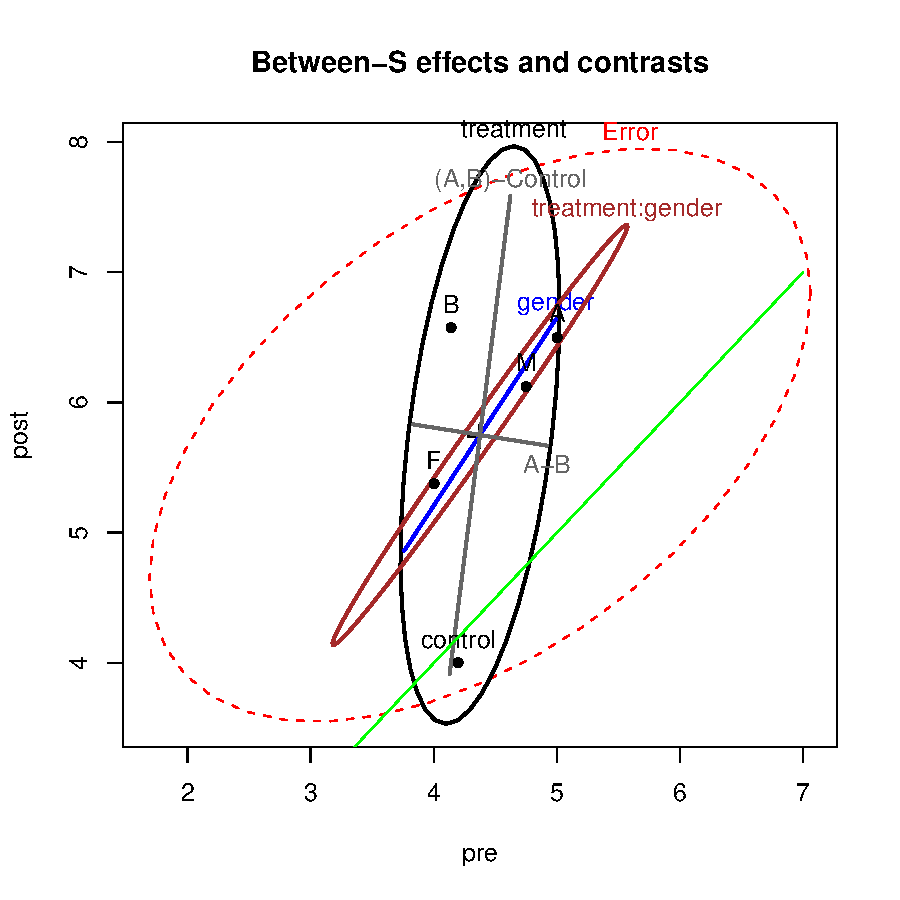
\includegraphics[width=1\linewidth,clip]{fig/plot-obk-HE1}
 \end{minipage}%
 \hfill
 \begin{minipage}[c]{.49\linewidth}
  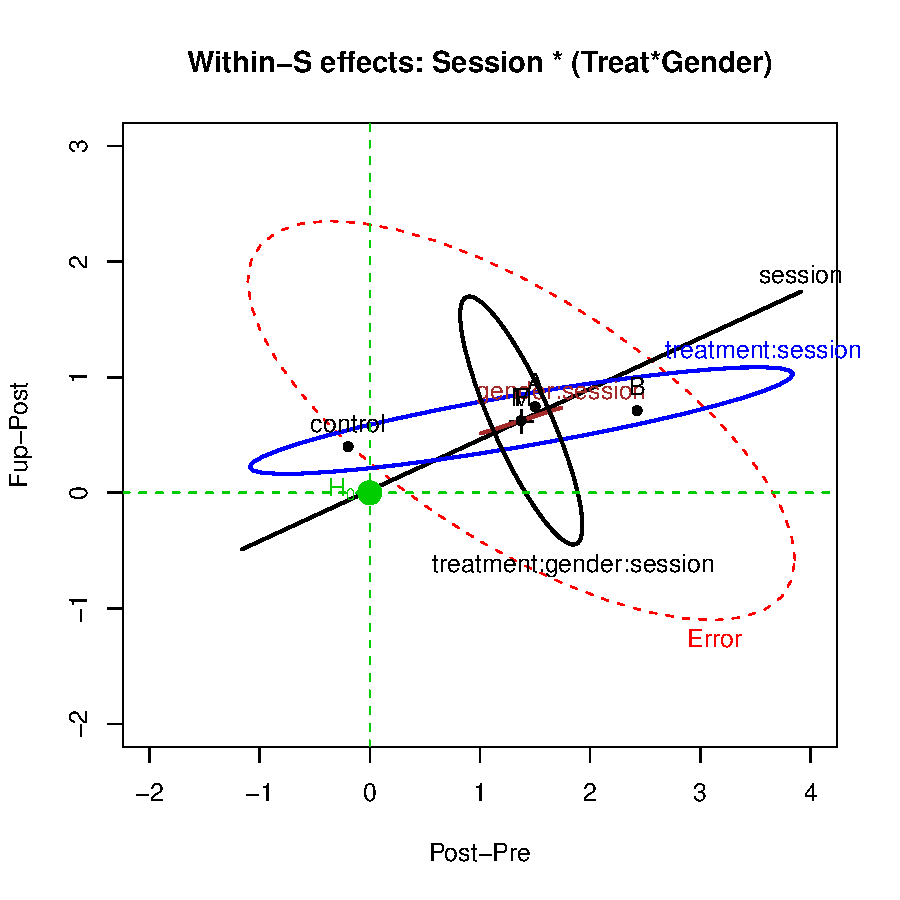
\includegraphics[width=1\linewidth,clip]{fig/plot-obk-HE3}
 \end{minipage}
\end{center}
\end{frame}
